\section{Computational details}
\label{app:computation}

\subsection{Configuration, records, and implementation names}

The numerical study has four environments, nine methods, and 160 paired
replications per environment, for 5,760 runs of 20,000 physical pulls.
The main table displays six methods; the cost--area figure and
Table~\ref{tab:allocation} include all nine. The additional path figure
below uses the same six methods as the main path figure.

The local reproducibility materials contain the complete configuration,
run-level records, saved paths, summary statistics, and paired differences
in \texttt{experiments/results/}. The configuration gives every arrival
time and mean, each method's parameters, and the seed mechanism. For
replication seed $s$ in environment index $j$, the generator is NumPy
PCG64 initialized with \texttt{SeedSequence([s,j])}, where
$s=202610150,\ldots,202610309$ and $j=0,\ldots,3$.
The resulting Bernoulli potential streams are shared across methods.
The policy uses only observed rewards and current arrivals. Array
preallocation is simulation storage and does not expose future arms or
the evaluation endpoint to a policy.

The reporting configuration is named Checkpoint-UCB in the article.
For reproducibility, its unchanged reference interface is
\texttt{CheckpointUCBAA} in \texttt{reference\_cp\_ucb\_aa.py}.
The experiment driver is \texttt{run\_experiments.py}.
The data IDs \texttt{CP-FIFO-fine}, \texttt{CP-FIFO},
\texttt{CP-confidence}, and \texttt{CP-period8} retain their existing
meaning. In particular, the first two are FIFO service every second pull
with $\rho=.04$ and $.12$; the latter two change allocation as specified
in the main article. The remaining IDs are \texttt{UCB-checkpoint},
\texttt{UCB-prefix}, \texttt{Growing-MOSS},
\texttt{ALL-epsilon-adapt}, and \texttt{Batch100-UCB}.
The ALL-$\varepsilon$ rule is a specified retained-history adaptation,
not a reproduction of FAREAST or $(\mathrm{ST})^2$.

\texttt{runs.csv} records one row per environment, seed, and method,
including full-run label errors, both unresolved-area totals, service
counts and regret, final per-arm counts, and the regret components below.
\texttt{paths.npz} contains all nine methods' regret, unresolved counts,
cumulative area, and total unresolved counts on a common grid, with
every arrival included. This is a saved time grid, not a per-round action
log. \texttt{summary.csv} and \texttt{paired\_differences.csv} provide
the numerical summaries; the two table source files are generated from
these records. \texttt{figures/gen\_fig\_performance.py} is the plotting
and tabulation entry point.

\begin{table}[t]
\centering
\caption{Allocation diagnostics. Each cell gives mean forced service pulls and mean final $\eta$-unresolved arms. UCB and MOSS have zero forced service.}
\label{tab:allocation}
\small
\begin{tabular}{lrrrr}
\toprule
Method & Stable & Improvements & Burst & Stop \\
\midrule
CP-FIFO ($\rho=.04$) & 10000, 8.00 & 10000, 6.00 & 10000, 5.00 & 10000, 5.00 \\
CP-FIFO ($\rho=.12$) & 7340, 0.16 & 5786, 0.00 & 5991, 0.00 & 5737, 0.00 \\
CP-confidence & 7144, 0.16 & 4653, 0.00 & 6092, 0.00 & 5322, 0.00 \\
CP-period8 & 2500, 6.74 & 2500, 0.20 & 2225, 3.00 & 2500, 2.00 \\
UCB-checkpoint & 0, 8.00 & 0, 3.00 & 0, 4.00 & 0, 4.00 \\
UCB-prefix & 0, 6.23 & 0, 0.11 & 0, 1.69 & 0, 1.71 \\
Growing-MOSS & 0, 7.00 & 0, 1.00 & 0, 4.00 & 0, 4.00 \\
ALL-$\varepsilon$ adapt. & 3696, 0.00 & 10000, 0.00 & 7794, 0.00 & 10000, 0.00 \\
Batch100-UCB & 0, 6.40 & 0, 0.53 & 0, 4.00 & 0, 2.89 \\
\bottomrule
\end{tabular}
\end{table}


\begin{figure}[p]
\centering
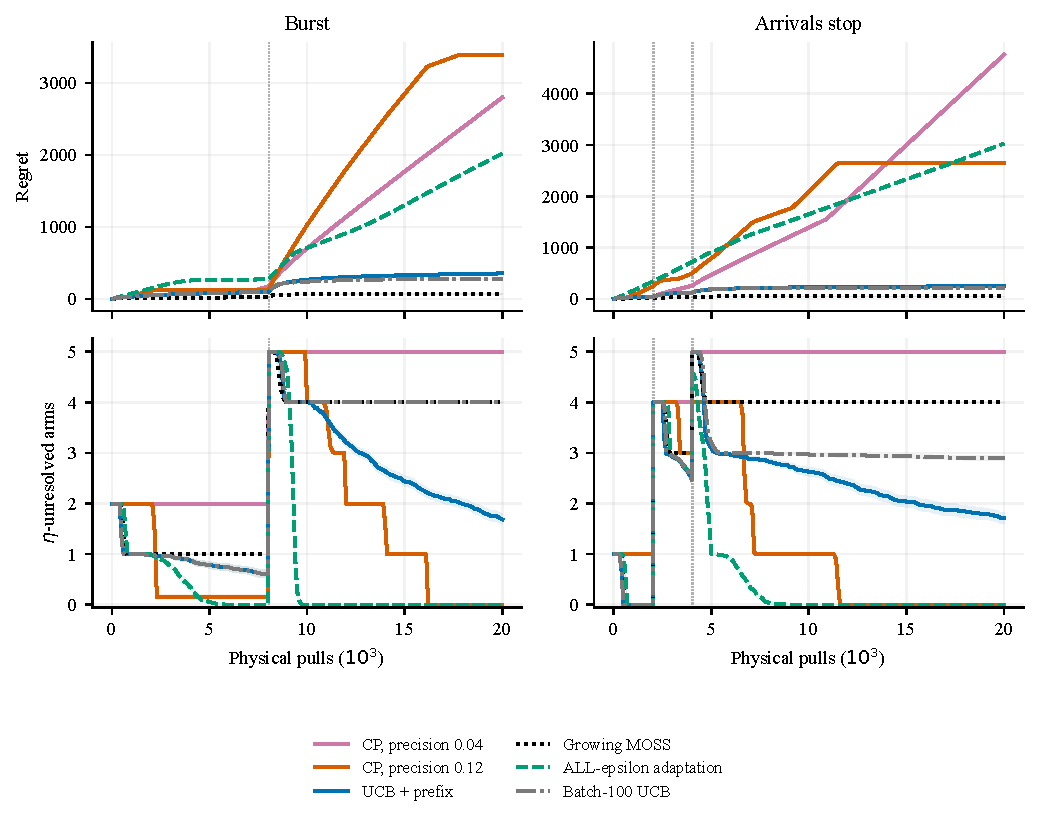
\includegraphics[width=.98\textwidth]{figures/fig_paths_pair2.pdf}
\caption{Additional paths for the burst and stopped-arrival environments.
The six displayed policies, common potential reward streams, 160
replications, and 1.96 Monte Carlo standard error bands are the same as
in the main path figure. Vertical lines mark actual arrivals. The full
run-level data and saved paths retain all nine policies.}
\label{fig:paths-additional}
\end{figure}

\subsection{Admission and reward-retirement accounting}

Let $\mathcal A_t^{\rm adm}\subseteq\mathcal A_t$ be the arms admitted
for reward selection, and let $B_t\subseteq\mathcal A_t^{\rm adm}$ be
its nonempty reward-active subset. Assume $I_t\in B_t$. Adding and
subtracting the admitted and active best means at each physical pull gives
the pathwise identity
\begin{equation}
\begin{aligned}
R_T={}&\sum_{t\le T}\bigl(\max_{i\in B_t}r_i-r_{I_t}\bigr)\\
&+\sum_{t\le T}\bigl(r^*(t)-\max_{i\in\mathcal A_t^{\rm adm}}r_i\bigr)
+\sum_{t\le T}\bigl(\max_{i\in\mathcal A_t^{\rm adm}}r_i
                         -\max_{i\in B_t}r_i\bigr).
\end{aligned}
\label{eq:three_part}
\end{equation}
The components are within-active learning, admission delay, and the
historical-retirement deficit. They are all nonnegative. In Batch100-UCB,
admission occurs at pulls $1,101,201,\ldots$, before action selection.
Reward retirement uses the confidence comparison among currently
admitted active arms after the current observation. Reporting continues
to cover all physically arrived arms, with $[0,1]$ intervals before
admission. Neither waiting for admission nor reward retirement is itself
a certificate of membership or nonmembership in the near-optimal set.

For Checkpoint-UCB, every arrived arm is immediately reward-eligible,
and negative reporting does not remove it from reward selection.
Thus $B_t=\mathcal A_t^{\rm adm}=\mathcal A_t$, so the last two
components vanish identically. The same statement applies to the other
immediate-admission methods that retain every arm for reward selection.

In the Batch100-UCB records, the admission contributions are $0$, $33.92$,
$16.00$, and $22.40$ for the stable, improving, burst, and stopped-arrival
environments, respectively. No retirement deficit occurred. Across all
5,760 records, the largest absolute difference between regret and the
sum in \eqref{eq:three_part} is below $3.1\times10^{-12}$.

\subsection{Verification and computational resources}

The production manifest records Python 3.11.7, NumPy 1.26.4, Numba 0.59.0,
Windows 10, and 13.5 seconds for production generation and recording,
excluding initial compilation and subsequent plotting. The resource snapshot records
20 physical CPU cores, 28 logical cores, and 31.71 GB system memory.
The small physical-round loops use compiled CPU execution. A detected GPU
was not needed. Dependencies and hashes of the reference implementation,
driver, configuration, and numerical records accompany the materials.

The saved production parity check compared the compiled FIFO procedure
with the reference interface for 20,000 consecutive rounds, checking
actions, service indicators, available-arm counts, and reports. That is a
historical implementation check. In this revision, separate short
deterministic checks compare the same interfaces around arrivals, quota
crossings, frozen intervals, and negative reports. The revision also
recomputes the 24 main-table rows, the complete allocation table, and the
640 all-unresolved finer-checkpoint records from the saved data.
These operations leave the simulation records and policy code unchanged.
They are implementation and accounting checks, rather than new method
comparisons or probability certificates.

The local materials support these resource and reproducibility
descriptions. A public repository or permanent release identifier has not
been verified for this version.
